% tex project for exam of Experimental Methods For High Energy Physics 
\documentclass[10pt]{beamer}

\usetheme[progressbar=frametitle]{metropolis}
\usepackage{appendixnumberbeamer}

\usepackage{booktabs}
\usepackage[scale=2]{ccicons}

\usepackage{pgfplots}
\usepgfplotslibrary{dateplot}

\usepackage{xspace}
\newcommand{\themename}{\textbf{\textsc{metropolis}}\xspace}

\usepackage{subfig}

\title{CMS Electromagnetic Calorimeter}
\subtitle{Design and HL-LHC Upgrade}
\date{\today}
\author{Daniele Brambilla}
\institute{University of Milano Bicocca}


\begin{document}



\maketitle    


\begin{frame}{Table of contents}
  \setbeamertemplate{section in toc}[sections numbered]
  \tableofcontents%[hideallsubsections]
\end{frame}

\section[LHC and the CMS experiment]{LHC and the CMS Experiment}

\begin{frame}[fragile]{The LHC}
    \begin{figure}
        \centering
        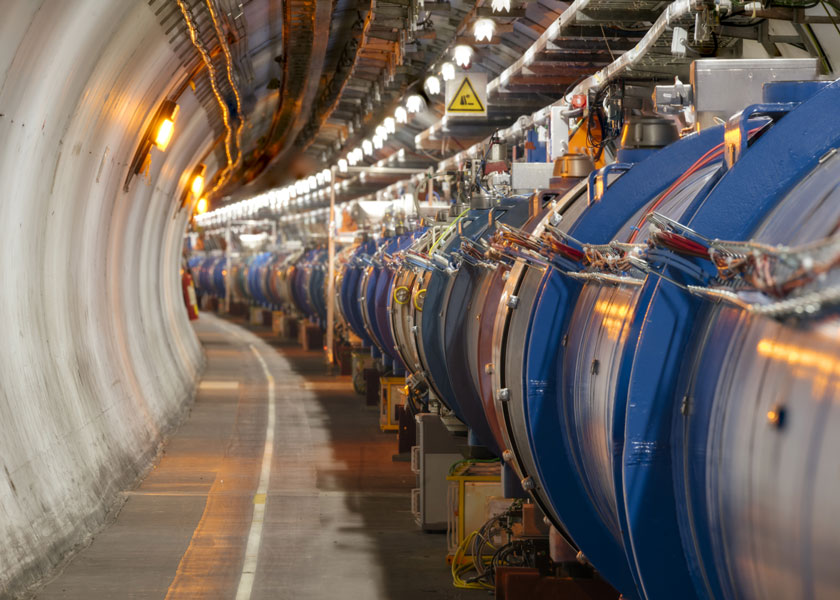
\includegraphics[width=.95\textwidth]{./img/CERN_LHC_tunnel.jpg}
    \end{figure}
\end{frame}

\begin{frame}[fragile]{CMS}
  \begin{figure}
        \centering
        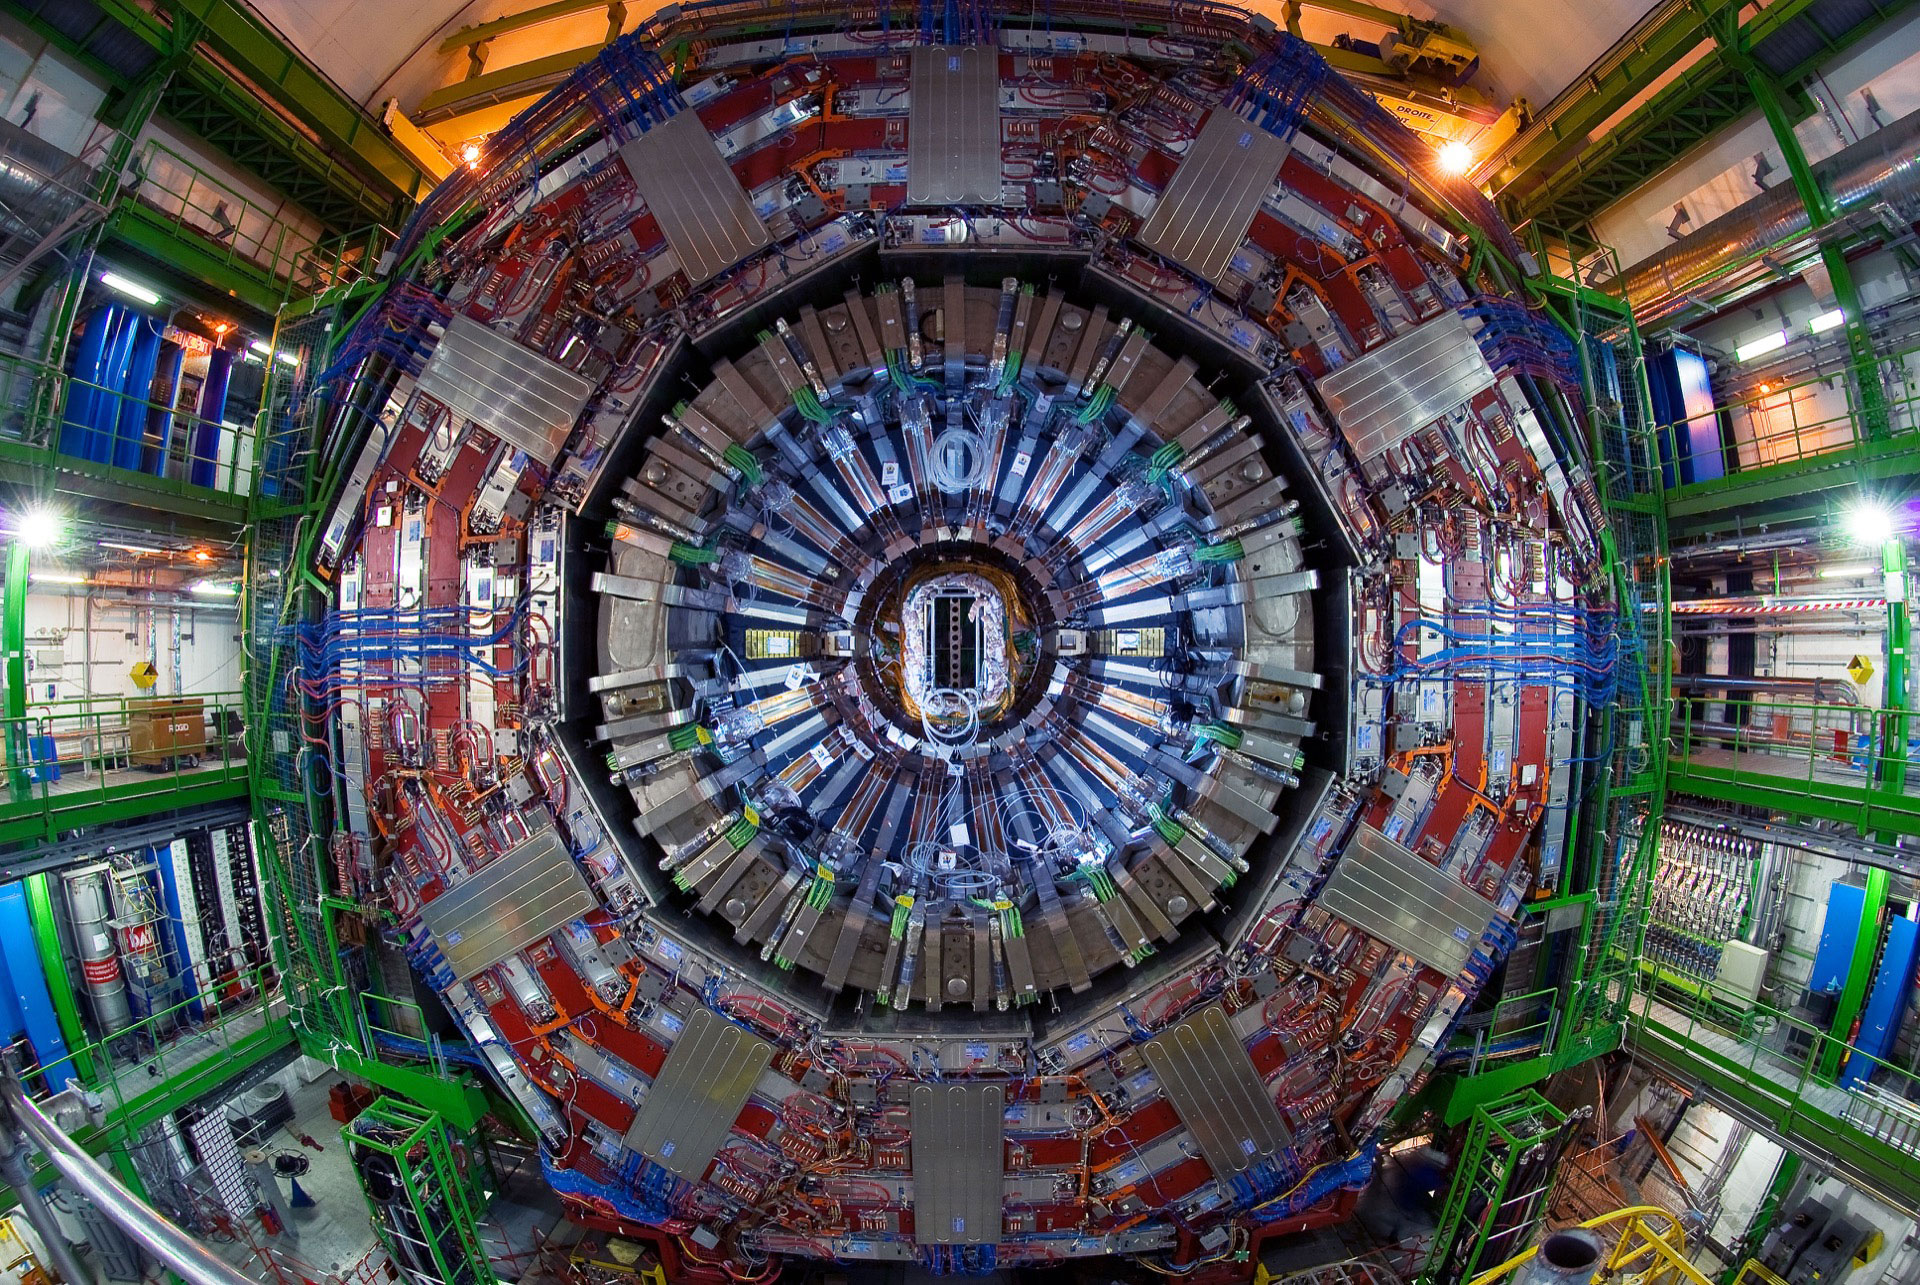
\includegraphics[width=.95\textwidth]{./img/CMS_front.jpg}
    \end{figure}
\end{frame}

\begin{frame}[fragile]{CMS}
  \begin{figure}
        \centering
        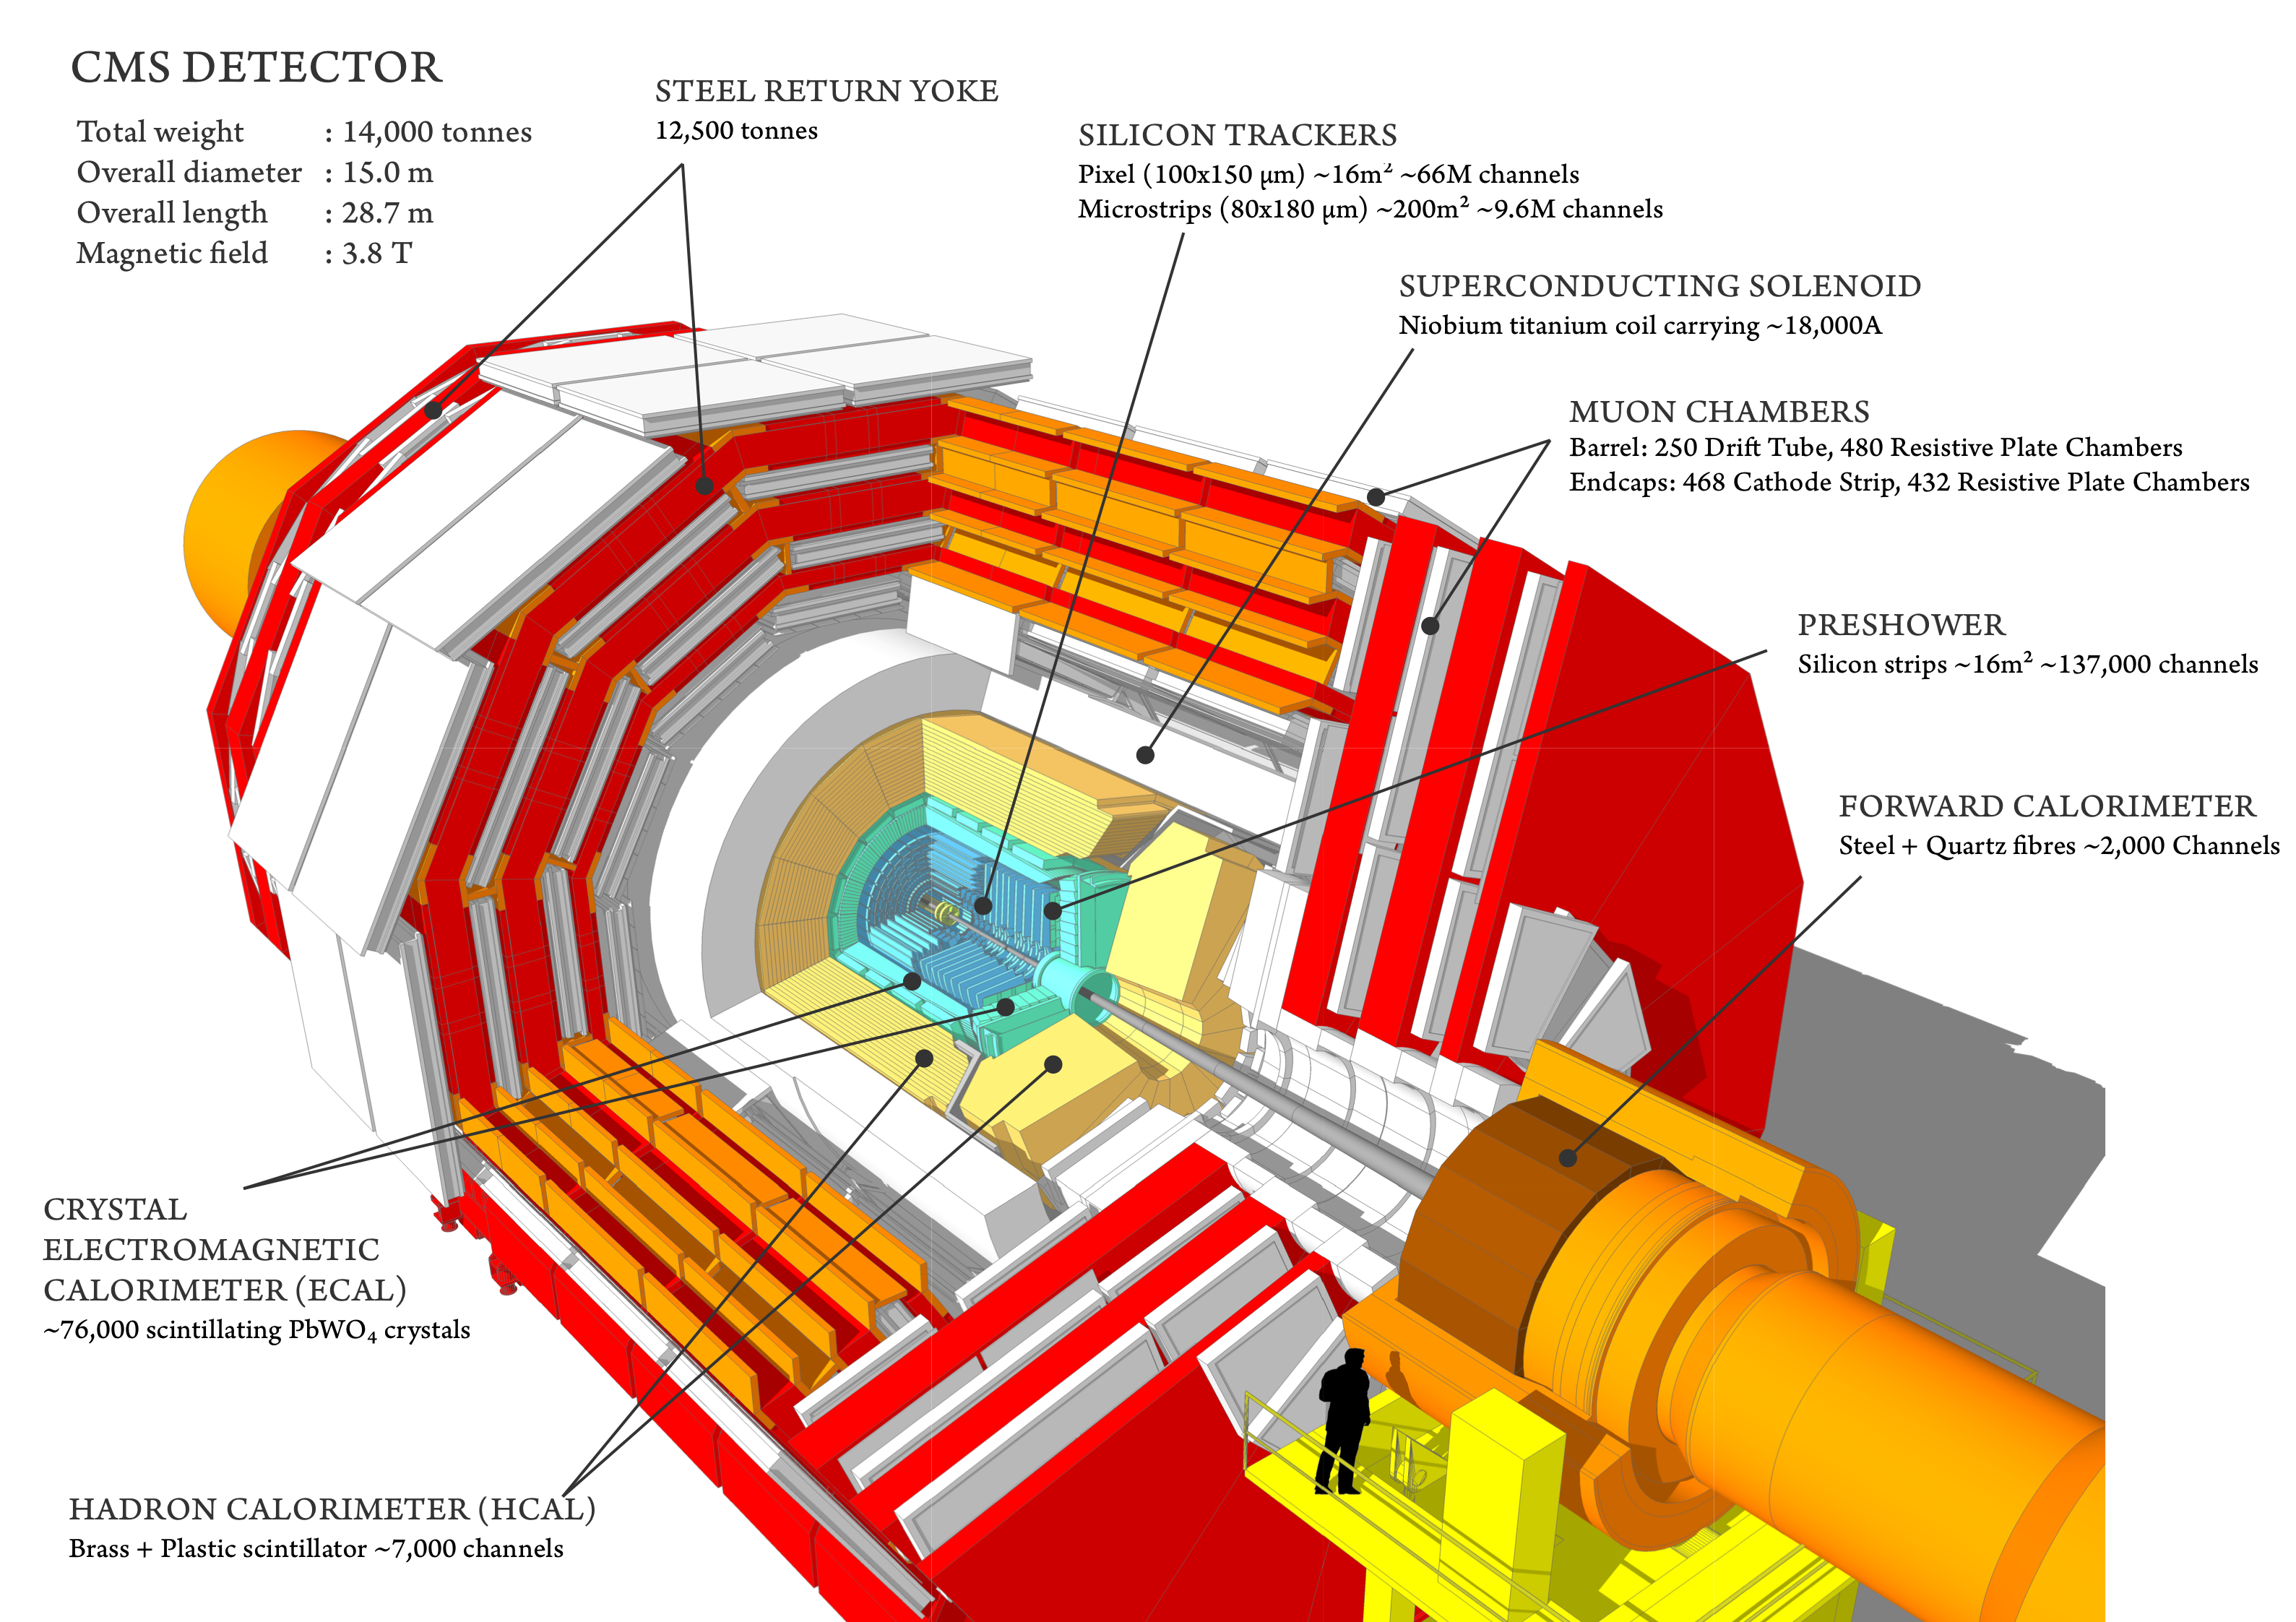
\includegraphics[width=0.95\textwidth]{./img/CMS_scheme.png}
    \end{figure}
\end{frame}


\section{Electromagnetic Calorimeter}

\begin{frame}[fragile]{EM Calorimeter}

    \textbf{Barrel ECAL}
    \begin{itemize}
        \item  covering $|\eta| \leq 1.479 $ range
        \item $61200$ crystals organized in $5\times5$ modules and $36$ supermodules
        \item $360$-fold in $\phi$ and $(2\times85)$-fold in $\eta$
        \item crystal lenght: $230$\,mm corresponding to $25.8\,X_0$ 
    \end{itemize}
    \textbf{Endcap ECAL} 
    \begin{itemize}
        \item $1.479 \leq |\eta| \leq 3.0 $
        \item Each endcap divided in 2 "Dees", each with 3662 crystals organized in $5\times5$ supercrystals
        \item crystal lenght: $220$\,mm corresponding to $24.7\,X_0$ 
    \end{itemize}
    \textbf{Pre-Shower Detector}
\end{frame}

\begin{frame}{EM Calorimeter Design}
    \begin{figure}
        \centering
        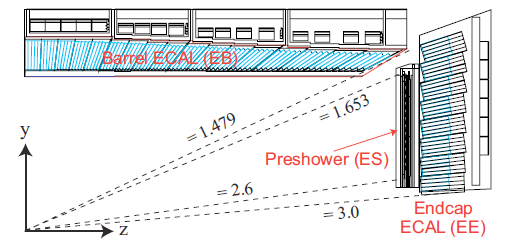
\includegraphics[width=\textwidth]{./img/EMCal_Scheme.png}
    \end{figure}
\end{frame}

\begin{frame}[fragile]{Barrel EM Calorimeter}
    \begin{figure}
        \centering
        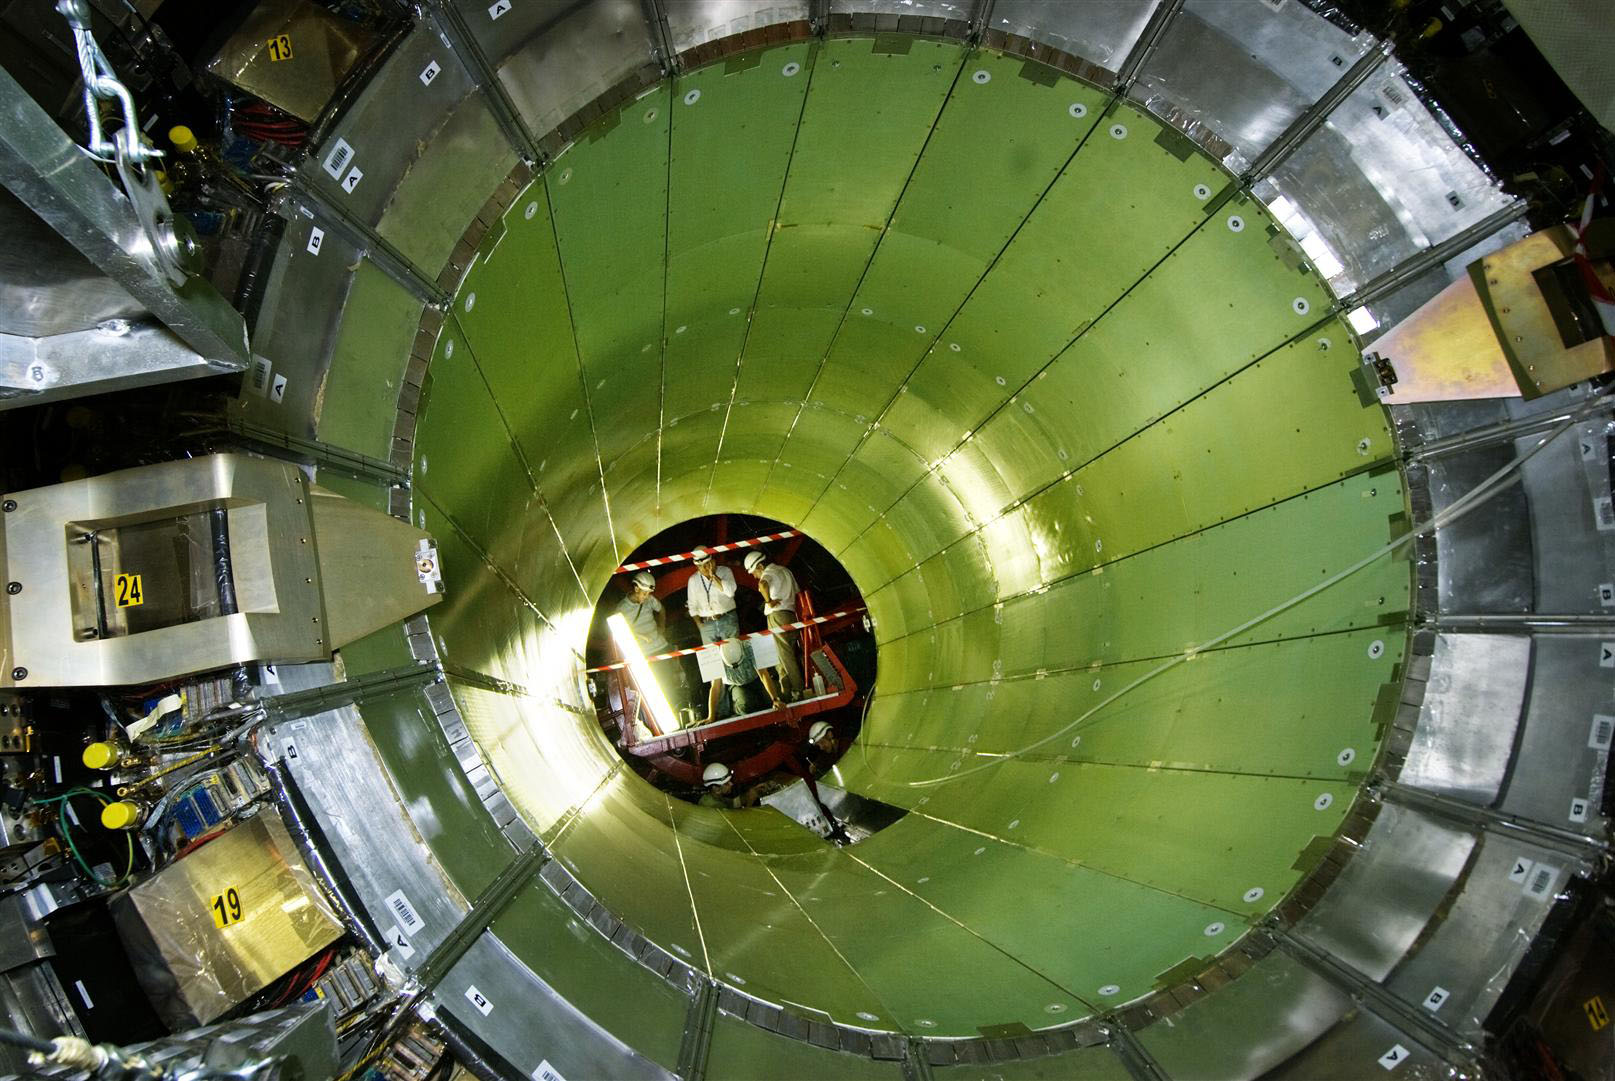
\includegraphics[width=\textwidth]{./img/ecal_barrel_photo.jpg}
    \end{figure}
\end{frame}

\begin{frame}{Endcap EM Calorimeter}
    \begin{figure}
        \centering
        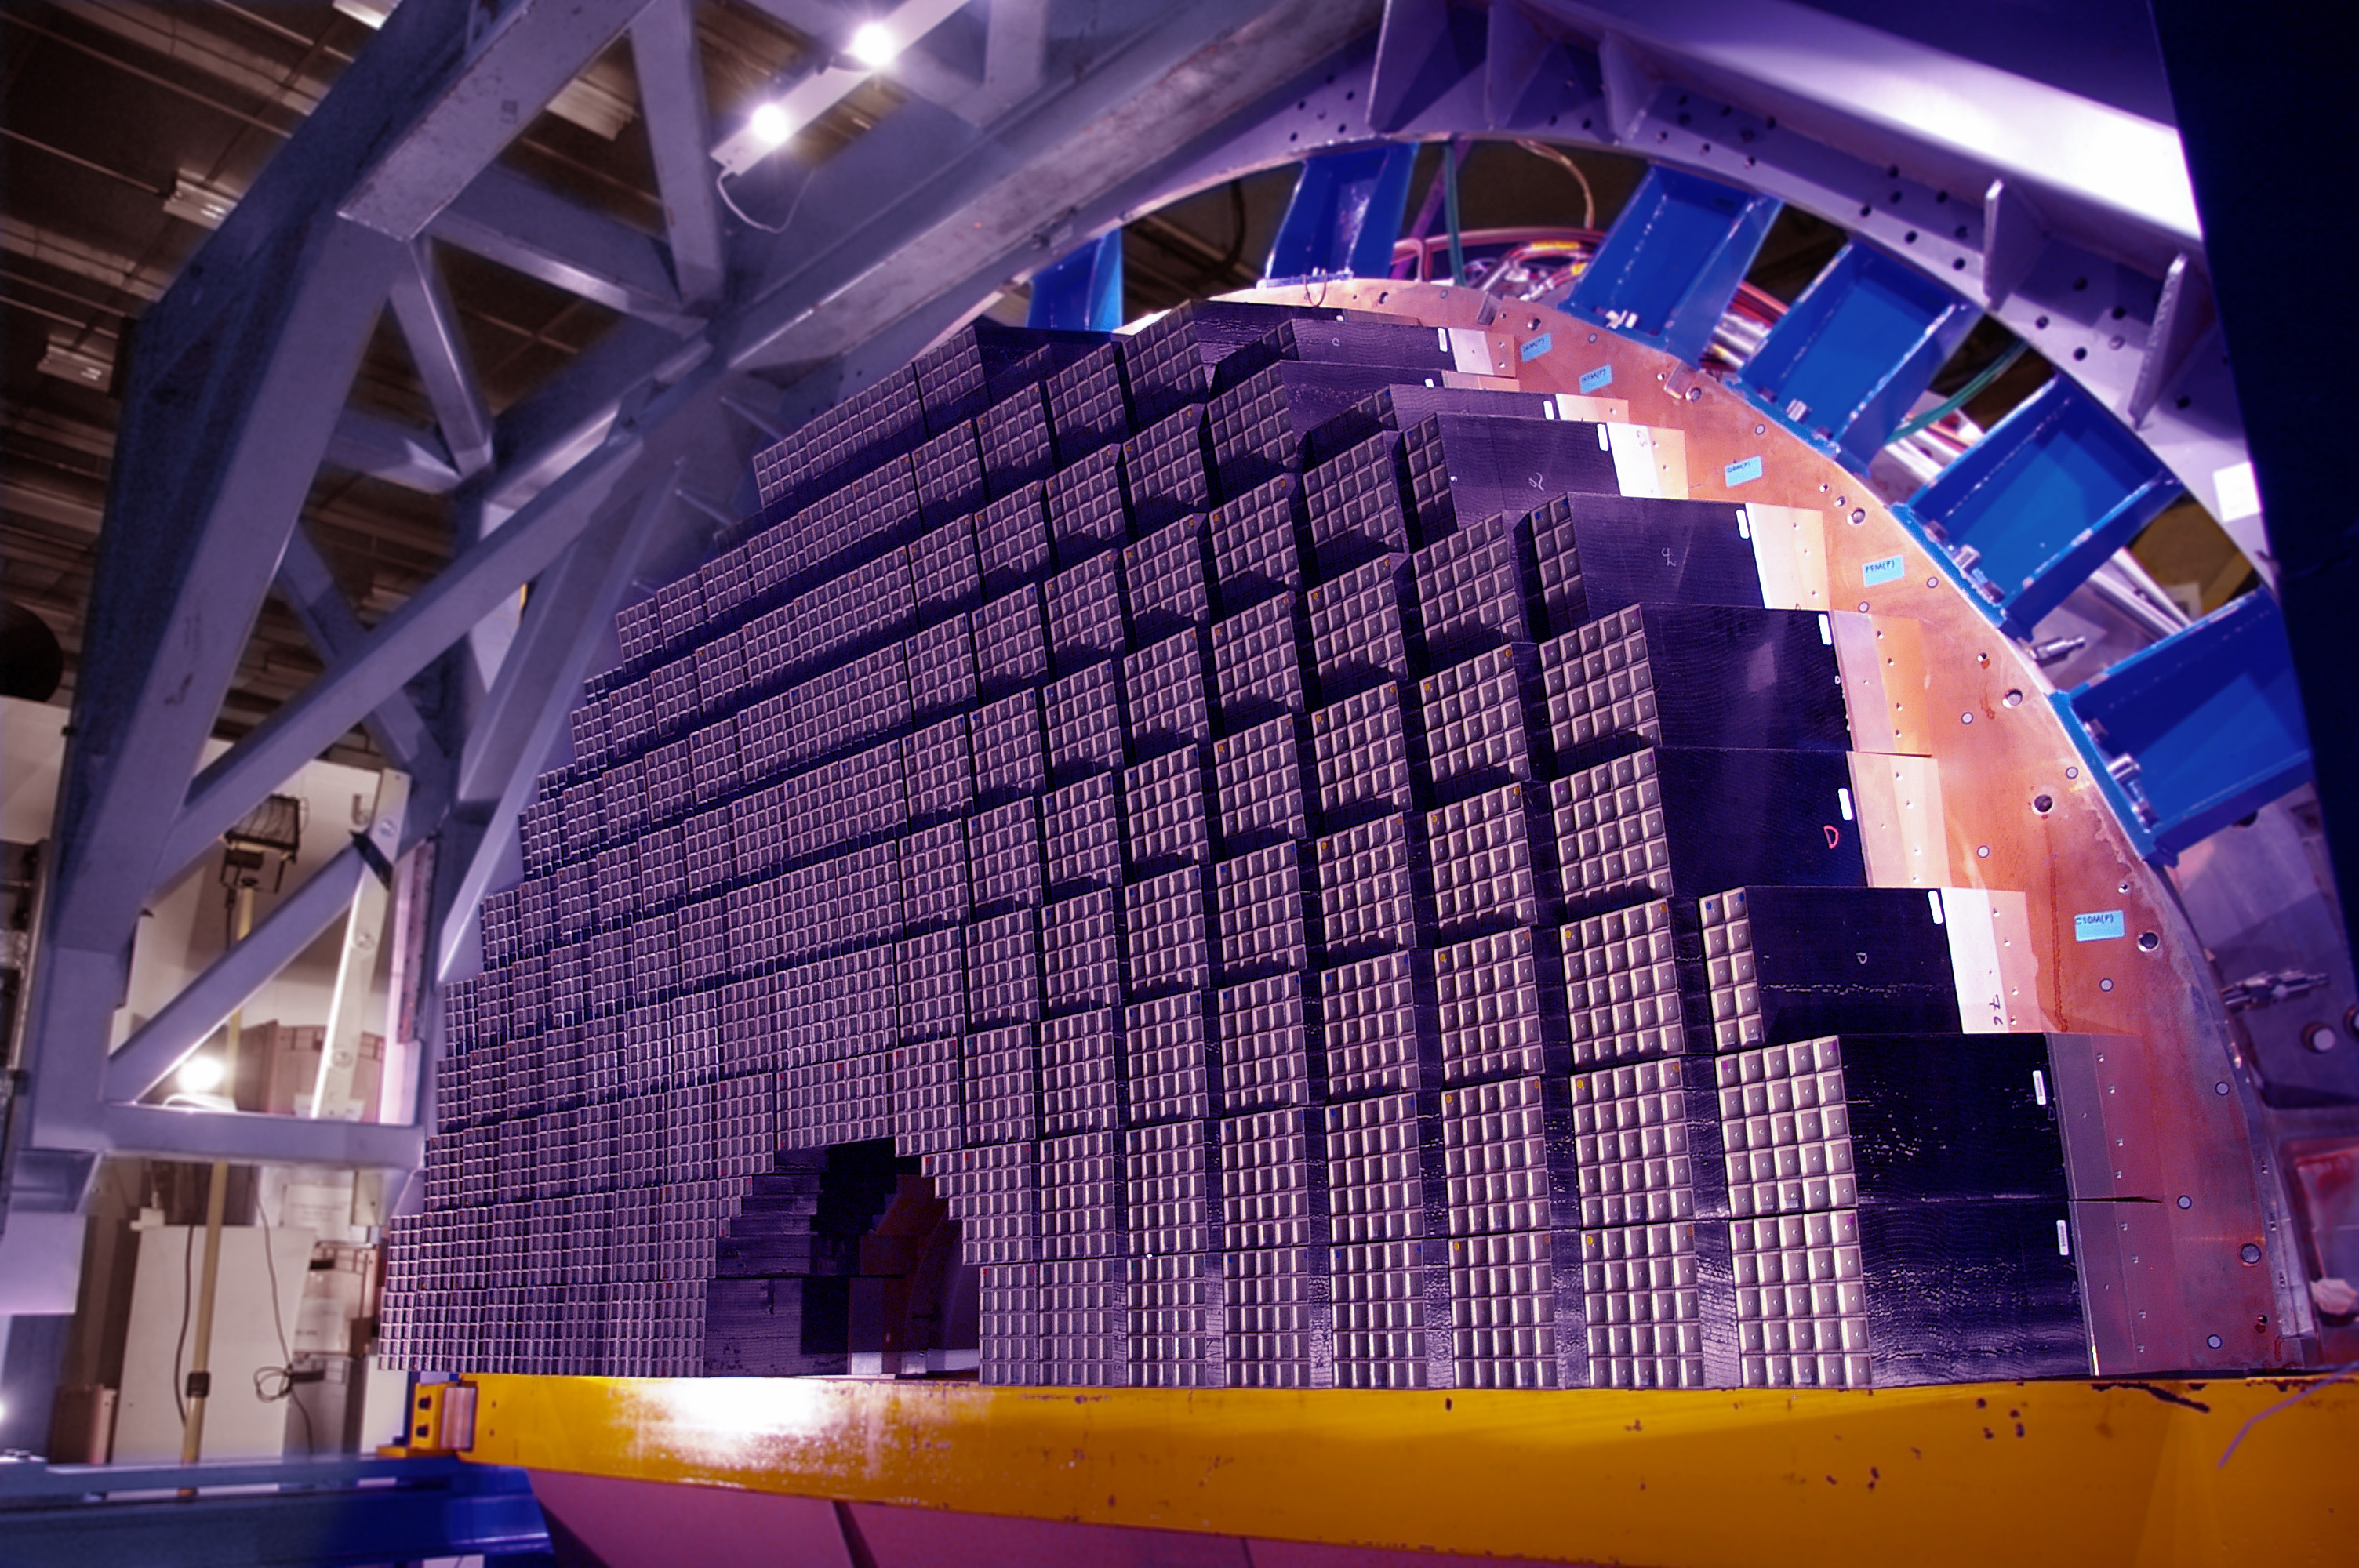
\includegraphics[width=\textwidth]{./img/ecal_endcap_photo.jpg}
    \end{figure}
\end{frame}

\begin{frame}{Lead Tungstate ($\text{PbWO}_4$) Crystals}
    \small{
    \begin{columns}
        \begin{column}[]{0.4\textwidth}
            \begin{figure}
                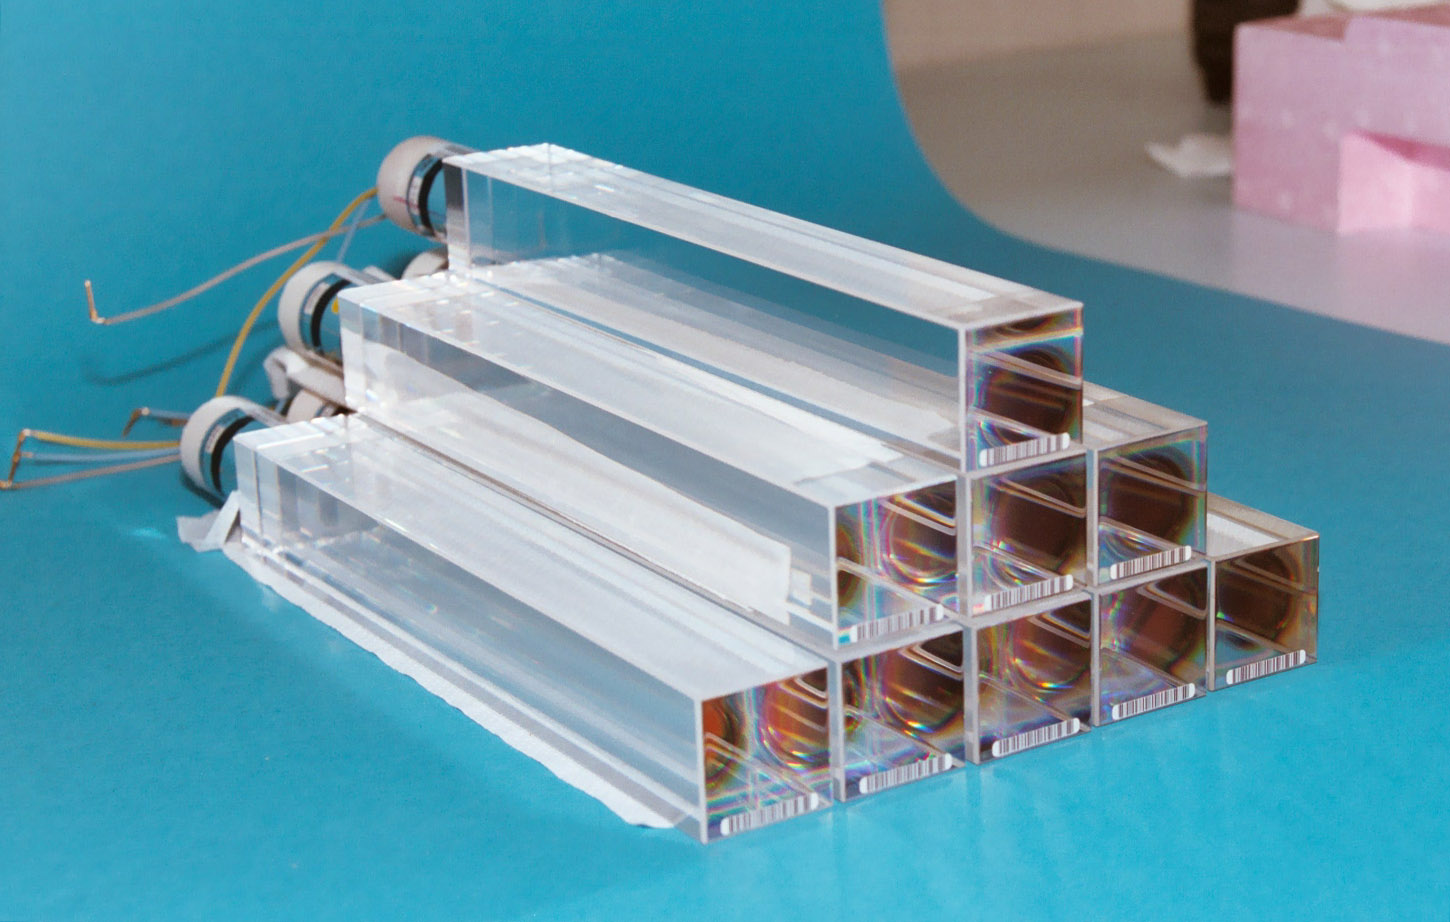
\includegraphics[width=\textwidth]{./img/crystals.jpg}
            \end{figure}    
        \end{column}
        \begin{column}[]{0.5\textwidth}
            \smallskip
            \begin{itemize}
                \item $\rho = 8.3\,$g/cm$^3$
                \item $X_0 = 0.89\,$cm
                \item Moliere Radius $ = 2.2$\,cm
                \item $2\times2\times25$\,cm (variable size) 
                \item Light Output: $4.5$ ph/MeV
                \item Green-Blue light, max @ 420\,nm
                %\item Polished for internal reflection
            \end{itemize}
        \end{column}
    \end{columns}
    \bigskip
    
    Exposure to \textbf{High radiation levels} causes the formation of \emph{absorption bands} and a wavelength dependent loss of light transmission, without changes to the scintillation mechanism.
    
    Radiation hardness properties are required: the induced light attenuation length must be always greater than 3$\times$ crystal length. 
    
    Damage is tracked and corrected by a laser light monitoring system.
    }
\end{frame}

\begin{frame}{Photodetectors}
    \textbf{Barrel EMCal}
    \begin{itemize}
        \item Reverse structure avalanche photodiodes (APDs)
        \item Glued to the back of the crystals
        \item High quantum efficiency ($\sim 75$\,\%) with mean gain of $50$
    \end{itemize}{}
    
    \textbf{Endcap EMCal}
    \begin{itemize}
        \item Vacuum Phototriodes
        \item Essentially photomultipliers, with a single gain stage
        \item Specially designed to withstand the $4$\,T magnetic field
        \item $22$\,\% quantum efficiency with mean gain around $10$ at $0$\,T
    \end{itemize}
\end{frame}

\begin{frame}{Pre-shower Detector}
    \textbf{Sampling calorimeter} with two layers: lead radiators with silicon strip sensors placed in between.
    Located in the \emph{forward region}, where the angle between couples of photons is more likely to be small, due to the boost of the $\pi_0$.
    
    Main purposes:
    \begin{itemize}
        \item principal aim: \textbf{neutral pions identifications} (from their decay products $\pi_0 \rightarrow \gamma \gamma$) within a fiducial region $1.653 < |\eta| < 2.6$  
        \item improve position determination of e and $\gamma$ due to its \textbf{finer granularity} (silicon strips $p\simeq2\,$mm).
        \item help electron identification against minimum ionizing particles.
    \end{itemize}{}
    
\end{frame}

\begin{frame}{Electronics and Signal}
    \textsc{\textbf{Front End Electronics}} located on-detector, made with radiation resistant circuits. Responsible of:
    \begin{itemize}
        \item Amplification and Shaping of the signal
        \item Digitization at $40\,$MHz
        \item Send information to trigger to be used for lv. 1 decisions
        \item Buffer data until reception of a lv. 1 trigger
        \item Transmit data to off detector electronics
    \end{itemize}{}
    \textsc{\textbf{Off Detector Electronics}} located in underground counting rooms
    \begin{itemize}
        \item Trigger System
        \item Readout of full-precision data and delivery to the Event Builder which builds data usable for analysis.
    \end{itemize}
\end{frame}

\begin{frame}{Amplitude Reconstruction}
    \textbf{Raw Data} is a series of consecutive digitizations at $40\,$MHz (Bunch Crossing Frequency).
    
    The simplest method for amplitude reconstruction is a sampling of the maximum of the pulse alone.
    
    Otherwise, one can use more samples:
    \begin{equation}
        \hat{A} = \sum_{i=0}^{i=N} w_i \times S_i ,
    \end{equation}
    where $S_i$ are the sample values and $w_i$ a series of weights. 
    
    Then algorithms can be applied for \emph{noise reduction} and \emph{out-of-time pile-up identification}.
\end{frame}

\begin{frame}{Energy Resolution}
    Showers in EMCal are reconstructed by building \emph{clusters} of crystals. Best performance is obtained using a 3x3 (or 5x5) sliding window centered in the crystal having the maximum energy deposition.
    \begin{figure}
        \centering
        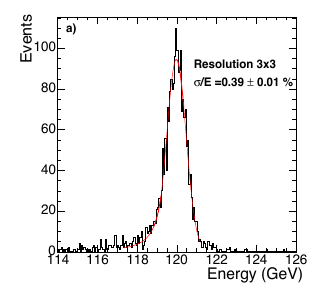
\includegraphics[height=130pt]{./img/resolution_1.png}
        \caption{Energy Distribution reconstructed during the test beam. The beam was pointed to the \textbf{center} of the supermodule).}
        \label{fig:res1}
    \end{figure}{}
\end{frame}

\begin{frame}{Energy Resolution}
    \begin{figure}
        \centering
        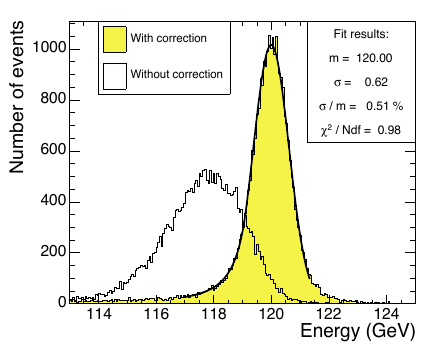
\includegraphics[height=150pt]{./img/resolution_2.png}
        \caption{Energy distribution reconstructed during the test beam. The beam was pointed to a \textbf{corner} of the supermodule. A single correction function, parametrized from the data, was applied to all regions of the supermodule to take into account variations in shower containment.}
        \label{fig:res2}
    \end{figure}{}
\end{frame}

\begin{frame}{Energy Resolution}
    Energy Resolution can be parametrized as a function of energy
    \begin{equation}
        \biggl(\frac{\sigma}{E}\biggr)^2 = \biggl(\frac{S}{\sqrt{E}}\biggr)^2 + \biggl(\frac{N}{E}\biggr)^2 + C^2 ,
    \end{equation}
  
    \begin{columns}
        \begin{column}[]{0.45\textwidth}
        \begin{itemize}
            \item S is the \textbf{stochastic} term
            \item N is the \textbf{noise} 
            \item C is a \textbf{constant} term, related to detector build quality and \emph{calibration}
        \end{itemize}
        \end{column}
        \begin{column}[]{0.45\textwidth}
            \begin{figure}
            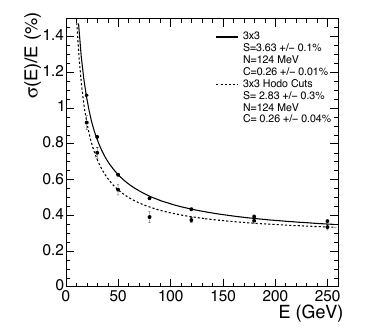
\includegraphics[width=\textwidth]{./img/res_energy.png}
            \end{figure}
        \end{column}
    \end{columns}
    
\end{frame}

\begin{frame}{Calibration}
    It is a \emph{severe technical challenge}.
    Naturally divided in two parts:
    \begin{itemize}
        \item \textbf{Absolute energy scale}
        \item \textbf{Inter-calibration} needed since single crystals have different scintillation light yield ($\sim 8\%$ RMS).
    \end{itemize}
    The final energy measurement is given by
    \begin{equation}
        E_{e,\gamma} = G \times \mathcal{F} \times \sum_i c_i \times A_i
    \label{eq:calib}
    \end{equation}
    where
    \begin{itemize}
        \item $G$ is a \emph{global absolute scale}
        \item $\mathcal{F}$ is a \emph{correction function} depending on particle type, position, $\eta$, momentum...
        \item $c_i$ are the \emph{inter-calibration coefficients}
        \item $A_i$ are the \emph{signal amplitudes} summed over the cluster of crystals 
    \end{itemize}{}
    
\end{frame}

\begin{frame}{Calibration}
    Various methods are used to obtain values for the parameters in equation \eqref{eq:calib}. These methods include:
    
    \begin{itemize}
        \item \textbf{Testbeam} precalibration.
        \item \textbf{Lab. Measurements} of the crystals light yield, giving a first estimate of the $c_i$ coefficients.
        \item \textbf{Phi independence} Taking advantage of the $\phi$ symmetry of deposited energy to inter-calibrate crystal rings at constant $\eta$.
        \item \textbf{Single electrons} Exploiting single electrons $p$ measurements from the \emph{tracker} to inter-calibrate different crystals in a single module.
        \item \textbf{Z $\rightarrow$ ee} Reconstruction of the ee invariant mass and calibration exploiting the Z mass constraint. 
%        Studying the distribution of 
%        \begin{equation}
%            \epsilon^i = \frac{1}{2} %\biggl[\biggl(\frac{M^i_\text{inv}}{M_Z}\biggr)^2 - 1\biggr]
%        \end{equation}
    \end{itemize}
    
\end{frame}

\begin{frame}{Phi Independence Method}
    \begin{figure}
        \centering
        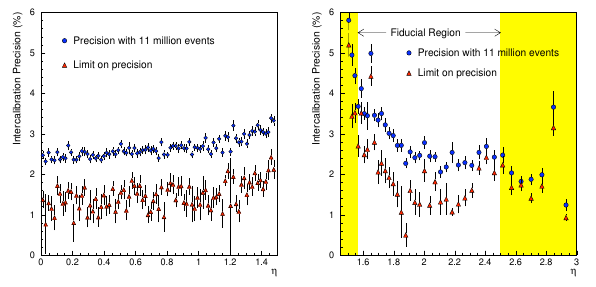
\includegraphics[width=\textwidth]{./img/intercalib_phi.png}
        \caption{Intercalibration precision as function on $\eta$, for barrel and endcap, for the \emph{phi-indipendence} method.}
        \label{fig:intercalib_phi}
    \end{figure}
\end{frame}



\begin{frame}{Single Electrons Method}
    \begin{figure}
        \centering
        \subfloat[][]{
            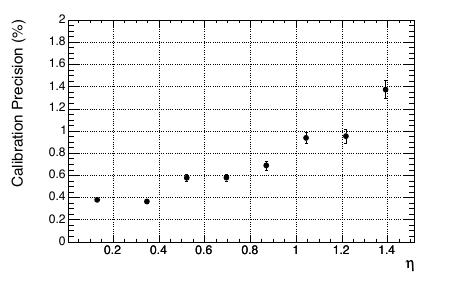
\includegraphics[width=.52\textwidth]{./img/single_e.png}
            } 
        \quad
        \subfloat[][]{
            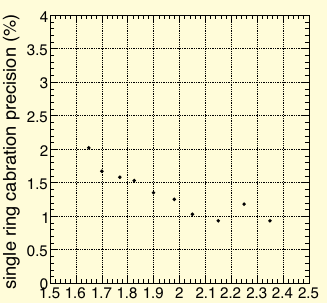
\includegraphics[width=.37\textwidth]{./img/single_e_endcap.png}
        }
        \caption{Calibration precision vs $\eta$ obtained with the single electrons method. (a) barrel case (b) endcap case.}
        \label{fig:single_electron}
    \end{figure}

\end{frame}

\begin{frame}{Z $\rightarrow$ ee Method}
    \begin{figure}
        \centering
        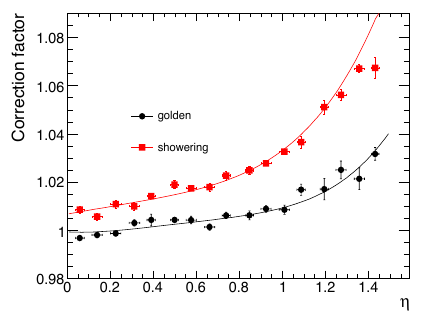
\includegraphics[width=.75\textwidth]{./img/Zee_corr_factor.png}
        \caption{Correction factor $\mathcal{F}$ \eqref{eq:calib} in dependence of $ \eta$, as extracted with the Zee method. \emph{Golden} comes from a MC simulation, \emph{showering} is obtained from $2\,\text{fb}^{-1}$ of Z $\rightarrow$ ee with intercalibration precision at $2\%$.}
        \label{fig:Zee_correction_factor}
    \end{figure}
\end{frame}

\section[High Luminosity LHC Upgrade]{High Luminosity LHC Upgrade}

\begin{frame}{High Luminosity LHC Upgrade}
    \begin{figure}
        \centering
        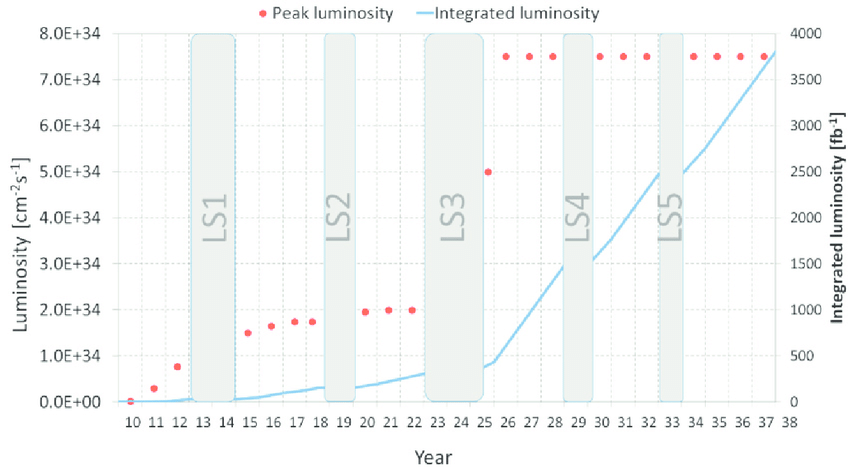
\includegraphics[height=150pt]{img/upgrade/luminosity.png}
    \end{figure}{}
    Objective: integrated luminosity $3000\,\text{fb}^{-1}$ ($10\times$ design value).
    
    Experimental challenges due to high \textbf{radiation} and higher \textbf{pileup}: detector upgrades are under development for every detector component.
\end{frame}

\begin{frame}{Calorimeters Upgrade}
    
    \begin{figure}
        \centering
        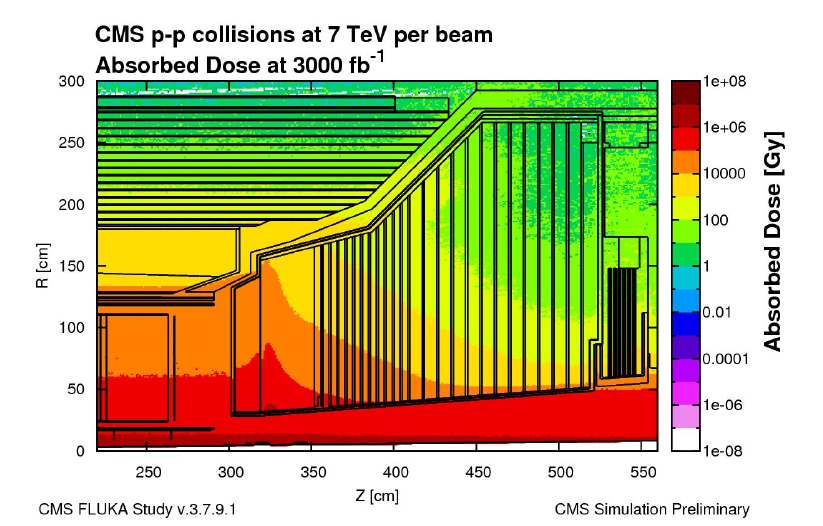
\includegraphics[height=150pt]{img/upgrade/doseRad.png}
    \end{figure}{}
    
    The \emph{endcap} calorimeters (HCal and EmCal) are exposed to the highest radiation dose, so will be entirely replaced.
\end{frame}

\begin{frame}{High Granularity Calorimeter}
    \begin{figure}
         \centering
         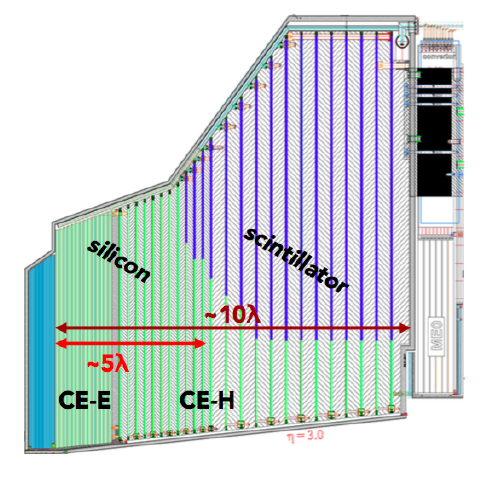
\includegraphics[height=180pt]{./img/upgrade/HGCalScheme.png}
         \caption{Schematic view of the High Granularity Calorimeter design.}
         \label{fig:my_label}
     \end{figure}{}
\end{frame}{}


\begin{frame}{High Granularity Calorimeter}
    It is a \textbf{sampling} calorimeter, consisting of an electromagnetic compartment (CE-E) followed by a hadronic compartment (CE-H).
    
    The ECAL and a large fraction of HCAL will be based on hexagonal silicon sensors of $0.5 - 1\,\text{cm}^2$ cell size, with the remainder of the HCAL based on highly-segmented plastic scintillators with SiPM readout.
    Absorber layers are made of Copper (EMCal) and Stainless Steel (HCal).

    The new HGCAL features:
    \begin{itemize}
        \item unprecedented transverse and longitudinal \textbf{segmentation} for both ECAL and HCAL compartments. 
        \item possibility of measuring the \textbf{Fine structure} of showers $\rightarrow$ better pileup rejection and particle identification
        \item high-precision \textbf{timing} capabilities thanks to silicon sensors
        \item \textbf{5D imaging} (x,y,z,t,E) through sophisticated algorithms 
    \end{itemize}{}
\end{frame}

%\begin{frame}{Conclusion}
%    \begin{flushright}
%        \emph{"Questo è quello che dicono... \\Poi, però, non funziona un ca**o!"}
%        
%        - cit. Luigi
%    \end{flushright}
%    \
%\end{frame}

\end{document}   

